
\chapter{Introduction}
It is becoming increasingly important to educate the public about their energy usage.  With the current state of alternative energy research, it is impossible to support the entire world on renewable energy.  In order to ensure that current energy sources are still available for future generations, organizations from non-profits to utility providers have advocated energy conservation.  Some organizations specifically target younger students in order to instill energy conservation habits as they transition to the real world.

One approach to educating the younger generation is to hold college dormitory energy competitions.  The goal of these competitions is to have the residents of the dorm reduce their energy usage.  Typically, the dorm that reduces their energy use the most at the end of the competition is declared the winner.  Other smaller prizes can be awarded for accomplishing certain goals, like reducing energy usage by 10 percent in a week.  The overall energy reduction is determined either by having someone read the meters or using "smart meters" that are connected to the internet and can send out data.  Universities such as Duke (Eco-lympics) and the University of Wisconsin (Energy Apocalypse) have run competitions relating to energy conservation and awareness. 

These competitions usually involve more than just reducing energy usage.  The competition organizers also include activities that relate to energy conservation and are geared toward improving energy literacy and awareness.  Examples of activities range from viewing documentaries relating to conservation to attending recycling drives.  Participation in these activities and encouraging others to do the same can also be recognized and rewarded in the context of these dorm energy competitions.

\section{The Problem}

To aid in running the competition, many of these universities used web sites to display the resident's current usage.  While it is easy to create a content management system to display mostly static data (i.e. one that is only updated when someone reads the meter), dormitory residents are more motivated by real-time feedback\cite{oberlin-feedback}.  However, the development of such a system can be a complicated and/or expensive process.  Providing real-time feedback not only requires special meters that can communicate with other devices, but also requires software that can process the data and display the relevant information to the user.  Because of this, many organizations have turned to companies like Lucid Design Group that can provide this software and hardware at a cost.

However, Lucid Design Group's software only involves the visualization of energy data and does not involve energy awareness activities.  It is designed to be embedded within a website rather than a complete competition package.  Because of this, the software is unable to immediately provide user-related information.  For example, if a dorm resident wants to view their floor's energy usage, they must interact with the visualization to get the information that they need.  In the ideal case, the user would log in using their university credentials and then be able to immediately view their current standings.

As for energy activities, this type of information can be posted on a website.  However, organizers would also like to be able to track interest and participation in these activities so that users can be rewarded.  Users also could be more motivated to participate if they see others in their floor/dorm participating.  Adding in these functions go beyond what a standard content management system does.  Developing such a module for a competition would also take more time and/or resources.

\section{Makahiki}

The goal of Makahiki is to provide a complete software package for organizations that want to hold their own dorm energy competitions.  It will have the following features:

\begin{enumerate}
	\item Integration with WattDepot as a source of energy data.
	\item Produce visualizations of the energy data retrieved from WattDepot.
	\item Support for Central Authentication Service (CAS) for logging in and logging out of the system.
	\item The ability to create and track participation in activities, commitments, and goals.
	\item Integration with social networks such as Facebook and Twitter for displaying progress and standings.
\end{enumerate}

WattDepot\cite{wattdepot} is an open source web service in development here at the University of Hawaii at Manoa.  Its purpose is to collect electricity data from sources and to store it.  By combining Makahiki with WattDepot, competition organizers have an automated way of tracking the energy usage for buildings.  While compatible meters still need to be purchased, the software comes at no additional cost.  WattDepot also provides data at near-real time intervals, meaning that dorm residents can immediately see the results of their actions.

While WattDepot is able to collect all of the electricity data, the data still needs to be processed and presented to users in a visually appealing way.  Through the use Google Visualizations, electricity data can be presented in a way that is easy to understand and dynamic.  Users will be able to see their past and current electricity usage and be able to compare it to other floors.  Competition standings and goal status can also be displayed to users.

Students nowadays have university computer accounts that they use to access their email and other electronic resources.  Universities typically implement this using a CAS login, which requires the student to log in through a central university server before accessing protected resources.  By leveraging this student authentication, we are able to present energy data in the context of their dorm or floor.  We can also present an interface for students to create their own profile and participate in activities.

Because competitions involve more than just reducing energy usage, Makahiki will also have support for creating activities, commitments, and goals.  Activities can range from replacing light bulbs in a desk lamp to attending meetings by sustainability organizations.  Commitments are typically small "pledges" that dorm residents can accept, like committing to turning off the lights in the lounge.  Goals are actions that entire dorm floors participate in.  Goals can include reducing energy usage by ten percent or having all the members of a floor attend an event.  Competition participants can participate in these items in order to gain points.

Furthermore, Makahiki will be configurable depending on the competition organizer's needs.  For instance, some organizations may wish to enter energy data manually since they cannot afford compatible smart meters.  Some organizations may wish to have a simple website for their competition without the added activities module.  These configurations are:

\begin{enumerate}
	\item Single page - A single page with news and charts.  The data for these charts can be either entered manually or retrieved from WattDepot.
	\item Tabbed interface - Includes sections for additional resources (i.e. links and videos) as well as energy data retrieved from WattDepot.
	\item Full Competition - Includes supplementary activities, commitments, and goals.  Also includes another tab for information about the competition.
\end{enumerate}

Finally, Makahiki will be open source.  This means that competition organizers can design the visual look of the application to fit their organization.  Also, advanced users can add or tweak modules in the application to fit their needs.

\section{Evaluating the Makahiki system}

The first step in evaluating the Makahiki system is to use it in our own dorm energy competition.  An initial version of Makahiki will be available for initial testing and review in the Summer of 2010.  Then, we will be holding a dorm energy competition here at the University of Hawaii at Manoa in October 2010 using both Makahiki and WattDepot.  Through the use of surveys, interviews, and/or log analysis, we hope to gain insight into how users will use the various features of Makahiki.

We also hope to provide an instance of Makahiki that looks similar to another dorm energy competition (for example, the Duke Eco-Olympics).  The purpose of this is to demonstrate the configuration options and how other universities can apply Makahiki to their own competition.

\section{Thesis Claims}

During the evaluation of Makahiki, we hope to answer the following questions:

\begin{enumerate}
	\item How effective is the site in influencing the energy usage habits of users?
	\item What components of Makahiki can we improve?
	\item How well does Makahiki support the potential needs of other energy competitions?
\end{enumerate}

\section{Proposal Structure}

Chapter 2 will discuss related works, which includes other dorm energy competitions.  Chapter 3 will describe the components of the Makahiki.  Chapter 4 describes our proposed evaluation procedure.  Finally, Chapter 5 includes the conclusion and provides a timeline for the work that is to be done to complete this project.

\chapter{Related Work}
\label{relatedwork}

The concept of holding dorm energy competitions is nothing new.  In fact, at least 25 institutions (including a private high school) have run dorm energy competitions.  This next section will discuss two of the more prominent dorm energy competitions; Duke and Oberlin.  We will then compare the features of the various universities.

\section{Other Dorm Energy Competitions}
\label{othercomps}

Duke held their first Eco-Olympics\cite{duke-eco-lympics} in 2002.  The Eco-Olympics not only involves energy conservation, but water conservation and waste reduction as well.  However, energy reduction plays a significant part in the competition as it is one of the largest components of the Eco-Olympics in terms of possible points.  Each week, the organizers get meter readings from the dorms and compare the readings with the dorm's respective baseline reading in order to calculate a per-capita reading.  This baseline reading is obtained in September, so it reflects usage when students are living in the dorm.   The key thing to note is that dorms are not directly competing against each other, as dorms vary in size and have differing energy requirements.  Also, the weekly readings are to provide feedback on how residents of each dorm are doing.  Points are only awarded at the end of the competition and the dorm with the lowest per-capita reading receives the full amount of points.

\begin{figure}[h]
	\includegraphics[scale=0.25]{images/duke-ecolympics.eps}
	\caption{Duke Eco-Olympics}
\end{figure}

The other major component of the Eco-Olympics is participation in events.  Dorms are awarded points based on the percent of residents who attend each event.  The amount of points for each event may vary, but the total points is comparable to the possible number of points for energy conservation.  These events can also involve conservation-related games.  The individuals participating in these games can also win prizes, providing additional incentive for dorm residents to participate.

Oberlin College in Ohio also runs dorm energy competitions.  Instead of going with manual meter readings, Oberlin has partnered with Lucid Design Group to create their Campus Resource Monitoring System\cite{oberlin-comp}.  The Campus Resource Monitoring System is active year-round and retrieves real time electricity and water usage from 26 buildings\cite{lucid-oberlin} on campus.  The system provides graphs and statistics and are presented to users in a clean and interactive way.

The first competition that used the Campus Resource Monitoring System proved to be a success.  A study conducted during the 2005 dorm energy competition found that dorms with real time feedback reduced their energy consumption by 55 percent while dorms with "medium resolution" feedback only reduced their energy usage by 32 percent\cite{oberlin-goals}.  In total, the competition saved 68,000 kW which translated to a savings of \textdollar5,100.

While Oberlin held yearly dorm energy competitions for some time, they had their first sustainability competition, called the Ecolympics, in March of 2008\cite{oberlin-history}.  The Ecolympics at Oberlin are run at about the same time as the dorm energy competition, but the two competitions are separate.  Dorms earn points for participation in events like attending environmentally themed lectures and film screenings\cite{oberlin-news}.  Depending on the event, participants can also win individual prizes.

\begin{figure}[h]
	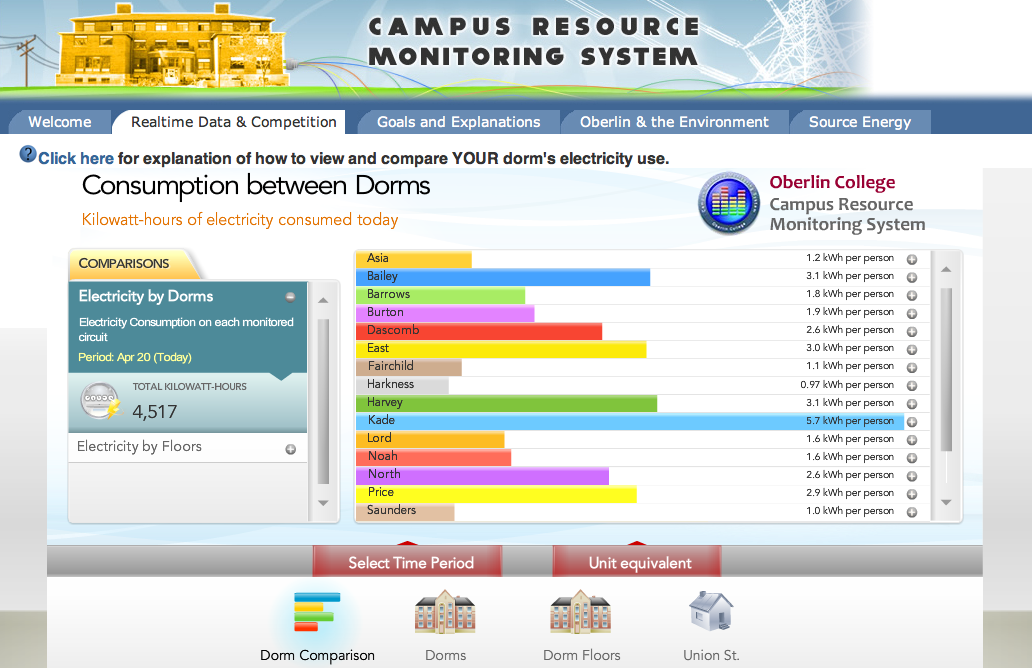
\includegraphics[scale=0.25]{images/oberlin-crms.eps}
	\caption{Oberlin College Campus Resource Management System}
\end{figure}

A few universities around the nation use Lucid Design Group's building dashboard for their dorm energy competition.  In addition to Oberlin College, Bowdoin College, St. John's University, Hamilton College, Boston College, and Elon University have all run dorm energy competitions through the use of Lucid Design Group's dashboard\cite{lucid-competitions} with great success.  Universities that do not use Lucid Design Group's dashboard typically go with a manual entry approach.  Because this requires direct access to the meters, the update interval can be as long as a week, providing dorm residents with very little feedback, if any at all.

\begin{table}[h]
	\begin{tabular}{|l||l|l|l|l|}
		\hline
		Organization & Year Started & Competition Duration & Update Frequency & Activities \\
		\hline
		Duke University & 2002 & 1 month & Weekly & Yes \\
		Oberlin College & 2008 & 2 weeks & Real-Time & Yes \\
		Brandeis University & 2006 & 2 weeks & Weekly & No \\
		Bowdoin College & 2002 & 1 month & Real-Time & No \\
		Harvard & 1990\cite{harvard-greencup} & 7 months & Manual & Yes \\
		Indiana University & 2008\cite{indiana-first} & 1 month & Manual & No \\
		\hline
	\end{tabular}
	\caption{University dorm energy competition implementations}
	\label{feature-matrix}
\end{table}

\chapter{Makahiki}
\label{makahiki}

\autoref{implementation} describes the implementation of the web application.  \autoref{wattdepot} goes into Makahiki's integration with WattDepot and the advantages of using WattDepot as a source of data.  \autoref{user} talks about what happens after a user logs in and the use of personalized information.  \autoref{activity} describes the activity framework and using it as a component of the dorm energy competition.  \autoref{mobile} describes how users with mobile devices such as Android phones or iPhones can interact with Makahiki. Finally, \autoref{socialint} describes Makahiki's integration with the Facebook social network.

\section{Implementation}
\label{implementation}

The current implementation of Makahiki is built using Django and Pinax.  Django\cite{django} is an open source web development framework implemented in Python.  Pinax\cite{pinax} is an open source platform built on Django that provides a set of reusable modules.  By using Pinax, we were able to start with a Django content management system and start building our unique modules right away.  Things like user accounts and profiles are created for us with little effort.

There are a few reasons why we chose Django and Pinax to implement Makahiki.  First, both are open source and thus other users who need to implement functionality can do so.  More importantly though, Django and Pinax provided us a lot of flexibility.  While we could have gone with a more popular content management system, these larger systems may not be flexible enough to support all of our needs.  Also, the process of extending such a large codebase would take additional time.  By going with Django, a general framework for creating web applications, we have the flexibility we desire.  And for the most part, we do not need to extend Django.  Instead, we just use the tools it provides to create the necessary modules for Makahiki.  Finally, Pinax provides starter implementations for different types of web applications.  For Makahiki, we started with a content management system project and gradually added some of the features in the social project.

With Pinax, we created a content management system for presenting sustainability-related information.  The content management system includes a news module where admins can create news stories to post on the front page.  Also, if Makahiki is receiving data from WattDepot, energy data from installed meters can also be presented in various ways. The content management system also includes space for information about the dorm energy competition and links to additional sustainability resources provided by administrators.

\section{WattDepot Integration}
\label{wattdepot}

WattDepot is an open source web service that collects and stores energy usage data from meters.  The system is currently under development in the Collaborative Software Development Laboratory at the University of Hawaii at Manoa.  While instances of the service are hosted in the laboratory, organizations can choose to host their own instances.

There are several reasons why we want to support integration with WattDepot.  First, the data in WattDepot is accessible via a REST API\cite{wattdepot-rest}, meaning that external services can easily request and retrieve data from the system.  Also, WattDepot supports near-real time (sub-minute) update intervals, which is one of the reasons why competitions that use Lucid Design Group's Building Dashboard are so successful.  With these updates, we can immediately present users with their current energy usage.  Users can then run "experiments", like seeing what happens when someone turns off their lights.  Other freely available solutions like Google PowerMeter\cite{google-powermeter} do not have this level of feedback.

Because WattDepot stores all of this data, Makahiki can retrieve current and historical data in order to provide visualizations.  Thus, competition participants can see how their usage has changed over time.  Administrators can also use this data to see if residents are completing energy reduction goals like reducing a floor's usage by 10 percent over a week.

\section{User Features}
\label{user}

Using Django's authentication framework, we also provide the ability for competition administrators and participants to log in to the website.  Instead of storing account information within Django, we chose to use a Django CAS plugin\cite{django-cas}.  With this plugin, users will be able to log in with the account provided to them by their organization (assuming that the organization hosts their own Central Authentication Service).  After users log in for the first time, they will also have the option to connect their account with Facebook using Facebook Connect.  Users will then be able to use their Facebook login to login to Makahiki.  Thus, Makahiki does not have to store any user passwords.

Once a user logs in, they will be taken to their profile.  Users will be able to add their own picture, insert their actual name, and some additional information about themselves.  Here, the user will also be able to view the latest activity for their floor.  A box that shows the user's current floor energy consumption will also be displayed as well as their current standings relative to other floors and/or dorms.

\section{Activity Framework}
\label{activity}

In addition to the energy conservation competition, we developed a framework for a separate competition based on points.  This competition requires users to participate in predefined tasks in order to earn points for their dorms and the dorm with the highest score wins.  This competition will typically be run at the same time as the dorm energy competition, as these tasks can provide competition participants with tips on how to reduce their energy usage.  The activity framework is split into three types of tasks: activities, commitments, and goals.

\subsection{Activities}

Activities are tasks that require a competition participant to perform a specific action in order to earn points.  Examples of activities include attending presentations, watching energy conservation related videos, or joining campus sustainability groups.  These activities are designed to make participants more knowledgeable and get them involved with the sustainability community.

Users who participate in activities usually require administrator approval before they can earn the points in the activity.  Administrators can either approve or reject these requests for points.  Makahiki supports three different confirmation types: question and answer, confirmation code, and image upload.

In the question and answer, the activity creator needs to come up with at least one question to ask participants.  The admin also specifies an answer to each question, which is merely used to help other administrators validate answers to questions.  When a participant requests to receive points for a question and answer activity, a random question is picked from the list of questions for that activity.  Once a participant submits their answer, it is then available for admins to review.  Activities that require participants to watch a video might require them to answer a question.  Questions can be as simple as "What is the unit of measurement for household energy?"

A confirmation code is typically used for activities that require attendance of an event.  The admin needs to specify the number of confirmation codes to generate.  Once the admin creates the activity, they can view the list of codes generated for this activity in a printable format.  When the event occurs, competition organizers can then hand out the confirmation codes to attendees of the event who are also participating in the competition.  When a participant requests points for this activity, they are required to enter a confirmation code.  If the code is valid, it is immediately approved.  Codes cannot be used more than once.  An example where a confirmation code might be used would be "Attend a free movie presentation of Planet Earth".

The image upload confirmation type requires participants to upload a picture in order to verify that they have performed the activity.  When the admin creates the activity, they also specify what the content of the image should be.  After the participant performs the activity, they are asked to upload the image.  Admins can then review the image.  An activity that might require an image upload would be "Replace an incandescent bulb with a CFL".  The participant could then be required to take a picture of themselves holding both the CFL and the incandescent bulb.

\subsection{Commitments}

Unlike activities, where a task is completed for points, commitments are more of a "pledge" to perform a task over a longer period of time.  Examples of commitments include "Turn off the lights in the bathroom when no one is using it" or "Make sure the lounge television is off when no one is there".  Commitments provide an incentive for users to change their energy usage habits.

Also, unlike activities, commitments do not require administrator approval.  Because of this, there are a additional constraints on commitments.  First, commitments are typically worth fewer points than activities.  Second, a user can only participate in up to five commitments, which prevents users from committing to every possible commitment.  Third, users who participate in commitments are public and displayed to fellow dorm floor residents, competition billboards, and on the web site.  Finally, participation in a commitment lasts for a week.  After this point, users can either participate in the same commitments or change to different commitments.

\subsection{Goals}

Goals are tasks that involve the participation of other dorm residents living on the same floor.  Examples of goals include "Reduce energy usage by 10%" or "Have everyone on the floor attend the Planet Earth movie screening".  Goals do not necessarily need to be "all or nothing"; partial points can be awarded if most of the dorm members participate in the goal.  These goals provide specific and measurable tasks that encourage members of the floor to work together.

Like commitments, a floor can only participate in a maximum of 5 goals.  This helps keep the floor focused on the goals they have at hand.  However, like activities, goals require administrator approval for points.  Because goals are typically connected to WattDepot or to other tasks in the activity framework, verification can be automated.  However, for our first release, we will keep things simple and have an administrator verify that the goal is completed.

\section{Billboard}
\label{billboard}

\section{Mobile Device Support}
\label{mobile}

Portable internet-connected devices like iPhones, iPod Touches, and Android phones are extremely popular nowadays.  Makahiki has support for custom view templates, including templates for mobile devices.  A default mobile template will provide competition participants with the ability to log in and view energy data.  Users will also be able to manage their participation in activities, commitments, and goals.

There are a few reason why we chose to go with a mobile formatted web site instead of a mobile application.  First, the support of multiple devices means that we need to develop multiple versions of the application.  A mobile application for the Android needs to be ported over to the iPhone. Second, mobile applications for iPhones, iPads, and iPod Touches need to be approved by Apple in order to be available for users.  An application can take a while to approve and even then we may need to resubmit the application multiple times.  Finally, a Makahiki application is just a way for a user to log in and see what is going on.  It does not require special device features such as GPS.

\section{Social Network Integration}
\label{socialint}

During our investigation of other dorm energy competitions, few organizations took advantage of popular social networks such as Facebook.  By integrating with Facebook, we allow users to share their activity within Makahiki with their friends.  As a result, Makahiki's potential influence expands from the dorm into each user's social graph.  For example, a user's Facebook friends may be encouraged to follow energy conservation tips that are posted by the user.  Also, students at other universities may be interested in hosting dorm energy competitions of their own based on the comments and activity of a current participant.

\chapter{Evaluation}
\label{evaluation}

Focus groups, surveys, actual competition.

\chapter{Conclusion}
\label{conclusion}

It is our hope that this system will improve the participants energy literacy in a way that makes a lasting impact on their energy use outside of the competition.

\section{Anticipated Contributions}

We want to provide a system that integrates real-time energy data along with incentives for behavioral change.

\section{Thesis Timeline}

\begin{enumerate}
\item August 2010 - An early version of the Makahiki will be available for evaluation.
\item October 2010 - The competition will take place.
\end{enumerate}